\documentclass[11pt]{article}
\usepackage[letterpaper, margin=1in]{geometry}
\usepackage{graphicx}
\usepackage{amsmath, amssymb}
\usepackage{booktabs}
\usepackage{hyperref}
\usepackage{caption}
\usepackage{subcaption}
\hypersetup{colorlinks=true, linkcolor=blue, urlcolor=blue}

% Figures are committed to docs/figures/ so the report compiles without running scripts.
\graphicspath{{../docs/figures/}}

\title{FiedlerEnsemble: Using Math to Detect Gerrymandering}
\author{Sohum Trivedi \and Ronit Kapoor \and Aditi Ghosh \and Maurya Bonu}
\date{NETS 1500, Spring 2026}

\begin{document}
\maketitle

\begin{abstract}
Gerrymandering is when politicians draw voting district boundaries to give
their party an unfair advantage. But how do you \emph{prove} a map is
gerrymandered rather than just oddly shaped? Our project answers this with
math. We treat each state as a network graph---where voting precincts are
nodes and shared borders are edges---and then generate thousands of
``neutral'' district maps using a computer. We measure how compact and
fair each map is, build a distribution of those measurements, and ask:
\emph{does the real enacted map look like an outlier?} If it falls deep
in the tail of the distribution, that is statistical evidence of
manipulation.

We analyze four states---Pennsylvania, North Carolina, Maryland, and
Wisconsin---using real precinct shapefiles and 2016 Presidential election
returns from the Metric Geometry and Gerrymandering Group (MGGG). Our
deterministic baseline uses a linear-algebra technique called the
\textbf{Fiedler vector} to produce a compact starting map. Our random
ensemble is generated by a \textbf{Metropolis--Hastings Markov chain}
that randomly swaps precincts between neighboring districts one at a
time. We score every map using five metrics for compactness and partisan
fairness, and report how unusual the real enacted map is compared to the
ensemble.
\end{abstract}

% -------------------------------------------------------------------
\section{Introduction: What Is Gerrymandering?}
\label{sec:intro}

Imagine you and your friends are dividing a pizza into slices, but you
get to decide where the cuts go---and you want the biggest slices for
yourself. Gerrymandering is like that, except the pizza is a state, the
slices are voting districts, and the goal is to get the most seats in
Congress for your party.

There are two main tricks. \textbf{Packing}: stuff as many of the
opposing party's voters as possible into a small number of districts,
so they ``waste'' votes winning by huge margins. \textbf{Cracking}:
spread the remaining opposing voters thin across many districts, so
they lose everywhere by small margins. The result: one party wins far
more seats than its statewide vote share would suggest.

Courts have struggled with gerrymandering because it is hard to formally
define ``too much'' partisan advantage---after all, some maps look
strange just because the underlying population is geographically
concentrated. The modern scientific approach is the
\emph{ensemble-comparison test} \cite{deford2021}: generate a large
random sample of neutral maps, measure partisan fairness on each one,
and check whether the real enacted map is a statistical outlier.

\paragraph{Our approach.} We implement this test from scratch for
four states. Our pipeline:
\begin{enumerate}
  \item Represents each state as a graph where precincts are nodes and
    shared borders are edges.
  \item Produces a high-quality starting map using a linear-algebra
    algorithm called spectral bisection.
  \item Randomly samples thousands of valid maps using a random-walk
    algorithm (MCMC).
  \item Scores every map using five metrics.
  \item Asks: how unusual is the enacted map compared to the
    random ensemble?
\end{enumerate}

All graph algorithms (spectral bisection, modularity, MST diameter,
MCMC, convergence diagnostics) are written by hand in Python.
NetworkX handles graph storage; SciPy provides the eigenvalue solver.

% -------------------------------------------------------------------
\section{Background: The Math Behind the Test}
\label{sec:bg}

\subsection{Representing a State as a Graph}

A \textbf{graph} $G = (V, E)$ is a collection of nodes $V$ and edges
$E$. Here:
\begin{itemize}
  \item Each \textbf{node} is one voting precinct (a small geographic
    unit, like a neighborhood).
  \item Each \textbf{edge} connects two precincts that share a physical
    border.
\end{itemize}

A redistricting plan divides all precincts into $k$ groups
(districts). A valid plan must satisfy three rules:
\begin{itemize}
  \item \textbf{Every precinct belongs to exactly one district.}
  \item \textbf{Each district must be geographically connected}---you
    should be able to drive from any precinct to any other precinct in
    the same district without leaving it.
  \item \textbf{Districts must have roughly equal populations}---within
    a tolerance $\tau$ of the ideal size $P / k$ (where $P$ is the
    state's total population).
\end{itemize}

The number of valid plans for a large state is astronomically large
(on the order of $10^{30}$ for Pennsylvania). So instead of looking at
all of them, we sample randomly.

\subsection{How We Measure Compactness}

A compact district looks like a blob or circle. A gerrymandered district
often looks like a snake or a squiggle. We use three graph-based
measures (no geometry needed, just the adjacency network):

\paragraph{Cut edge ratio.} If you draw lines between all neighboring
precincts that are in \emph{different} districts, the cut edge ratio is
the fraction of total edges that are cut:
\[
  \mathrm{Cut}(\mathcal{P})
  = \frac{\text{number of edges crossing district boundaries}}{\text{total edges}}.
\]
Compact districts have fewer cut edges because neighboring precincts
tend to be in the same district. A gerrymandered, tentacle-like map
cuts through many more edges.

\paragraph{MST diameter.} For each district, we build a
minimum spanning tree (MST)---the shortest network that connects all
its precincts---and measure how long (in hops) the longest path through
that tree is. A round, compact district has a small diameter; a long
thin district has a large one. We average this across all districts.

\paragraph{Newman--Girvan modularity.} Modularity $Q$ measures whether
districts follow the natural community structure of the graph---whether
precincts that are deeply interconnected tend to be in the same
district:
\[
  Q(\mathcal{P})
  = \sum_{i=1}^{k}
    \left[ \frac{e_{ii}}{m} - \left( \frac{d_i}{2m} \right)^2 \right],
\]
where $m$ is total edges, $e_{ii}$ is edges within district $i$, and
$d_i$ is the sum of degrees of precincts in district $i$. Higher $Q$
means the partition respects natural clustering. Gerrymandered maps that
break up communities will have lower modularity.

\subsection{How We Measure Partisan Fairness}

\paragraph{Efficiency gap.} Every vote cast for the losing candidate in
a district is ``wasted'' (it did not help elect anyone). Every vote cast
for the winning candidate above the 50\%+1 threshold is also wasted
(surplus votes that weren't needed). The efficiency gap counts
these wasted votes per party:
\[
  \mathrm{EG} = \frac{W_R - W_D}{V_{\text{total}}},
\]
where $W_R$ and $W_D$ are total wasted Republican and Democratic votes.
A positive EG means Republicans are wasting fewer votes and have a
structural advantage. Magnitudes above 0.07 are typically flagged as
extreme \cite{stephanopoulos2015}.

\paragraph{Mean--median difference.} In a fair map, the median district
partisan lean should be close to the mean. If packing has occurred, the
distribution of per-district Democratic vote share becomes skewed: a
few districts win overwhelmingly (packed) and many others lose narrowly.
This shows up as a gap between mean and median:
\[
  \mathrm{MM} = \overline{s_D} - \mathrm{median}(s_D),
\]
where $s_D$ is the vector of per-district Democratic vote shares.

\paragraph{Seats--votes curve.} We ask: if the statewide vote share
shifted by $\pm 20$ percentage points uniformly, how many seats would
each party win? A fair map produces a smooth S-curve through the
midpoint. A gerrymandered map produces an asymmetric curve---one party
``wins big'' on seat counts even at moderate vote advantages.

\subsection{Checking That Our Random Sampler Worked Properly}

Because our random ensemble is generated by a chain of random moves,
we need to check that the chain actually explored the full space of
valid maps (rather than getting stuck in one corner). We use two
standard diagnostics from statistics:

\paragraph{Gelman--Rubin $\hat{R}$.} We run three independent chains
from different random seeds. If they all converge to the same
distribution, the $\hat{R}$ statistic for each metric should be close
to 1.0. Values above 1.1 suggest the chains have not yet mixed.

\paragraph{Effective sample size (ESS).} Because consecutive maps in a
chain are correlated (each differs by only one precinct from the last),
900 consecutive samples contain less unique information than 900
independent draws. ESS estimates how many truly independent samples
we effectively have.

% -------------------------------------------------------------------
\section{Methods}
\label{sec:method}

\subsection{Step 1: Building the Precinct Graph}

We load real precinct shapefiles from the Metric Geometry and
Gerrymandering Group (MGGG) \cite{mggg}, which provides free,
MIT-licensed data for Pennsylvania, North Carolina, Maryland, and
Wisconsin. Each precinct shapefile contains the precinct polygon
geometry, total population (from the 2010 Census), and 2016
Presidential election vote counts (Democratic and Republican).

We project all shapefiles to NAD83 / Conus Albers (EPSG:5070), a
standard projection for the contiguous United States that preserves
area measurements. Two precincts become neighbors (connected by an
edge) if their polygons share a border of non-trivial length.
``Island'' precincts that share no border with any other precinct are
stitched to their nearest neighbor by centroid distance.

\subsection{Step 2: The Spectral Baseline Plan (Fiedler Vector)}

Before random sampling, we need a good starting map. Starting from a
random map would waste thousands of steps just reaching a valid,
balanced partition. Instead, we use a mathematical technique called
\textbf{spectral bisection}.

Every graph has a matrix called the \textbf{Laplacian} $L = D - A$,
where $A$ is the adjacency matrix (1 if two nodes are neighbors, 0
otherwise) and $D$ is a diagonal matrix of node degrees. The Laplacian
encodes the connectivity structure of the graph. Its eigenvectors
reveal natural ways to partition the graph.

The \textbf{Fiedler vector} $\mathbf{f}$ is the eigenvector
corresponding to the second-smallest eigenvalue of $L$. Sorting
precincts by their value in $\mathbf{f}$ and cutting at a threshold
gives an approximate minimum cut---a natural division of the graph into
two parts that preserves internal connectivity. We apply this
recursively to get $k$ districts.

\paragraph{Handling non-power-of-two district counts.} A naive
recursive halving fails when $k$ is not a power of two (e.g.,
Pennsylvania has $k = 18$ districts). We use a \emph{proportional}
split: when dividing a piece that will become $k_t$ districts, the
Fiedler cut puts $\lfloor k_t/2\rfloor / k_t$ of the population on the
left. This ensures all final districts have approximately equal
population even for any $k$.

\paragraph{Fixing disconnected districts.} After recursive bisection,
some districts may be disconnected (a precinct island split off from the
main body). We repair this by reassigning small disconnected fragments
to whichever neighboring district shares the most boundary edges with
the fragment.

\subsection{Step 3: Random Sampling via MCMC}

Starting from the spectral baseline, we generate thousands of random
valid maps using a \textbf{single-flip Metropolis MCMC} sampler. The
idea: at each step, pick a random edge on the boundary between two
districts, and propose moving the precinct on one side of that edge
into the other district. Accept the move only if it keeps every
district contiguous and within the population tolerance. Record the
current map every 30 steps after a 3{,}000-step warm-up period.

\begin{figure}[h]
\hrule\medskip
\noindent\textbf{Algorithm: Single-flip Metropolis MCMC}
\medskip\hrule\medskip
\begin{tabbing}
xx \= xxx \= xxx \kill
1.\> Start from the spectral baseline map \\
2.\> for each step: \\
3.\> \> Pick a random edge crossing a district boundary \\
4.\> \> Propose flipping the precinct on the larger-population side \\
5.\> \> \textbf{Reject} if the source district becomes disconnected \\
6.\> \> \textbf{Reject} if either district's population leaves the $\pm 5\%$ band \\
7.\> \> Otherwise accept the flip \\
8.\> After warm-up, save a snapshot every 30 steps
\end{tabbing}
\hrule
\caption{One step of the MCMC sampler. Each saved snapshot is one
  sample in the ensemble.}
\end{figure}

We run 3 independent chains (different random seeds) for 300 saved
samples each, giving a pooled ensemble of 900 maps per state. We check
convergence with $\hat{R}$ and ESS.

\subsection{Step 4: Scoring and Outlier Detection}

We compute all five metrics on every map in the ensemble, building a
distribution for each metric. Then we compute the enacted plan's
metrics and ask where they fall. Specifically, we report:
\begin{itemize}
  \item The \textbf{percentile}: what fraction of ensemble maps have a
    more extreme value.
  \item A \textbf{two-sided $p$-value}: the fraction of ensemble maps
    at least as far from the ensemble median as the enacted map. A
    small $p$-value means the enacted map is unusual.
  \item A \textbf{95\% bootstrap confidence interval} on the $p$-value,
    constructed by resampling the ensemble 500 times.
  \item A \textbf{composite severity score}: the average of
    $-\log_{10}(p)$ across metrics. Higher means more extreme overall.
\end{itemize}

% -------------------------------------------------------------------
\section{Data}
\label{sec:data}

All data comes from the Metric Geometry and Gerrymandering Group
(MGGG) at \url{https://github.com/mggg-states}, which provides free,
MIT-licensed precinct shapefiles. No login or registration is required.

\begin{center}
\begin{tabular}{llrrll}
\toprule
State & MGGG repo & VTDs & Districts ($k$) & Election & Enacted plan \\
\midrule
Pennsylvania & PA-shapefiles & 9{,}253 & 18 & 2016 Pres. & 2018 Remedial (court-ordered) \\
North Carolina & NC-shapefiles & $\sim$2{,}700 & 13 & 2016 Pres. & 2016 Enacted \\
Maryland & MD-shapefiles & $\sim$2{,}000 & 8 & 2016 Pres. & 2011 Enacted \\
Wisconsin & WI-shapefiles & $\sim$1{,}900 & 8 & 2016 Pres. & 2011 Enacted \\
\bottomrule
\end{tabular}
\end{center}

VTD = Voting Tabulation District (the census name for a precinct-level
geographic unit). Population figures come from the 2010 decennial
census; vote totals are from the 2016 Presidential General Election.

\textbf{Context for the enacted plans:}
Pennsylvania's 2018 remedial plan was \emph{ordered by the state
Supreme Court} after the original 2011 map was struck down as an
unconstitutional partisan gerrymander. It is therefore expected to be
\emph{fairer} than a typical random map. North Carolina's 2016 map was
challenged for racial and partisan gerrymandering and later redrawn.
Maryland's 2011 map has long been considered one of the most aggressive
Democratic gerrymanders in the country. Wisconsin's 2011 map was struck
down by a federal district court (though later reversed on standing by
the Supreme Court).

% -------------------------------------------------------------------
\section{Results}
\label{sec:results}

For each state, the figure shows: (left) the enacted map and the
spectral baseline map, colored by district; (center) histograms of the
MCMC ensemble for four metrics with the enacted and spectral values
marked; (right) the seats--votes curve. All results use 900-plan
ensembles (3 chains $\times$ 300 samples, lag 30, burn-in 3{,}000,
population tolerance $\pm 5\%$).

\subsection{Pennsylvania: The Court-Ordered Fair Map}
\label{sec:pa}

\begin{figure}[h]
  \centering
  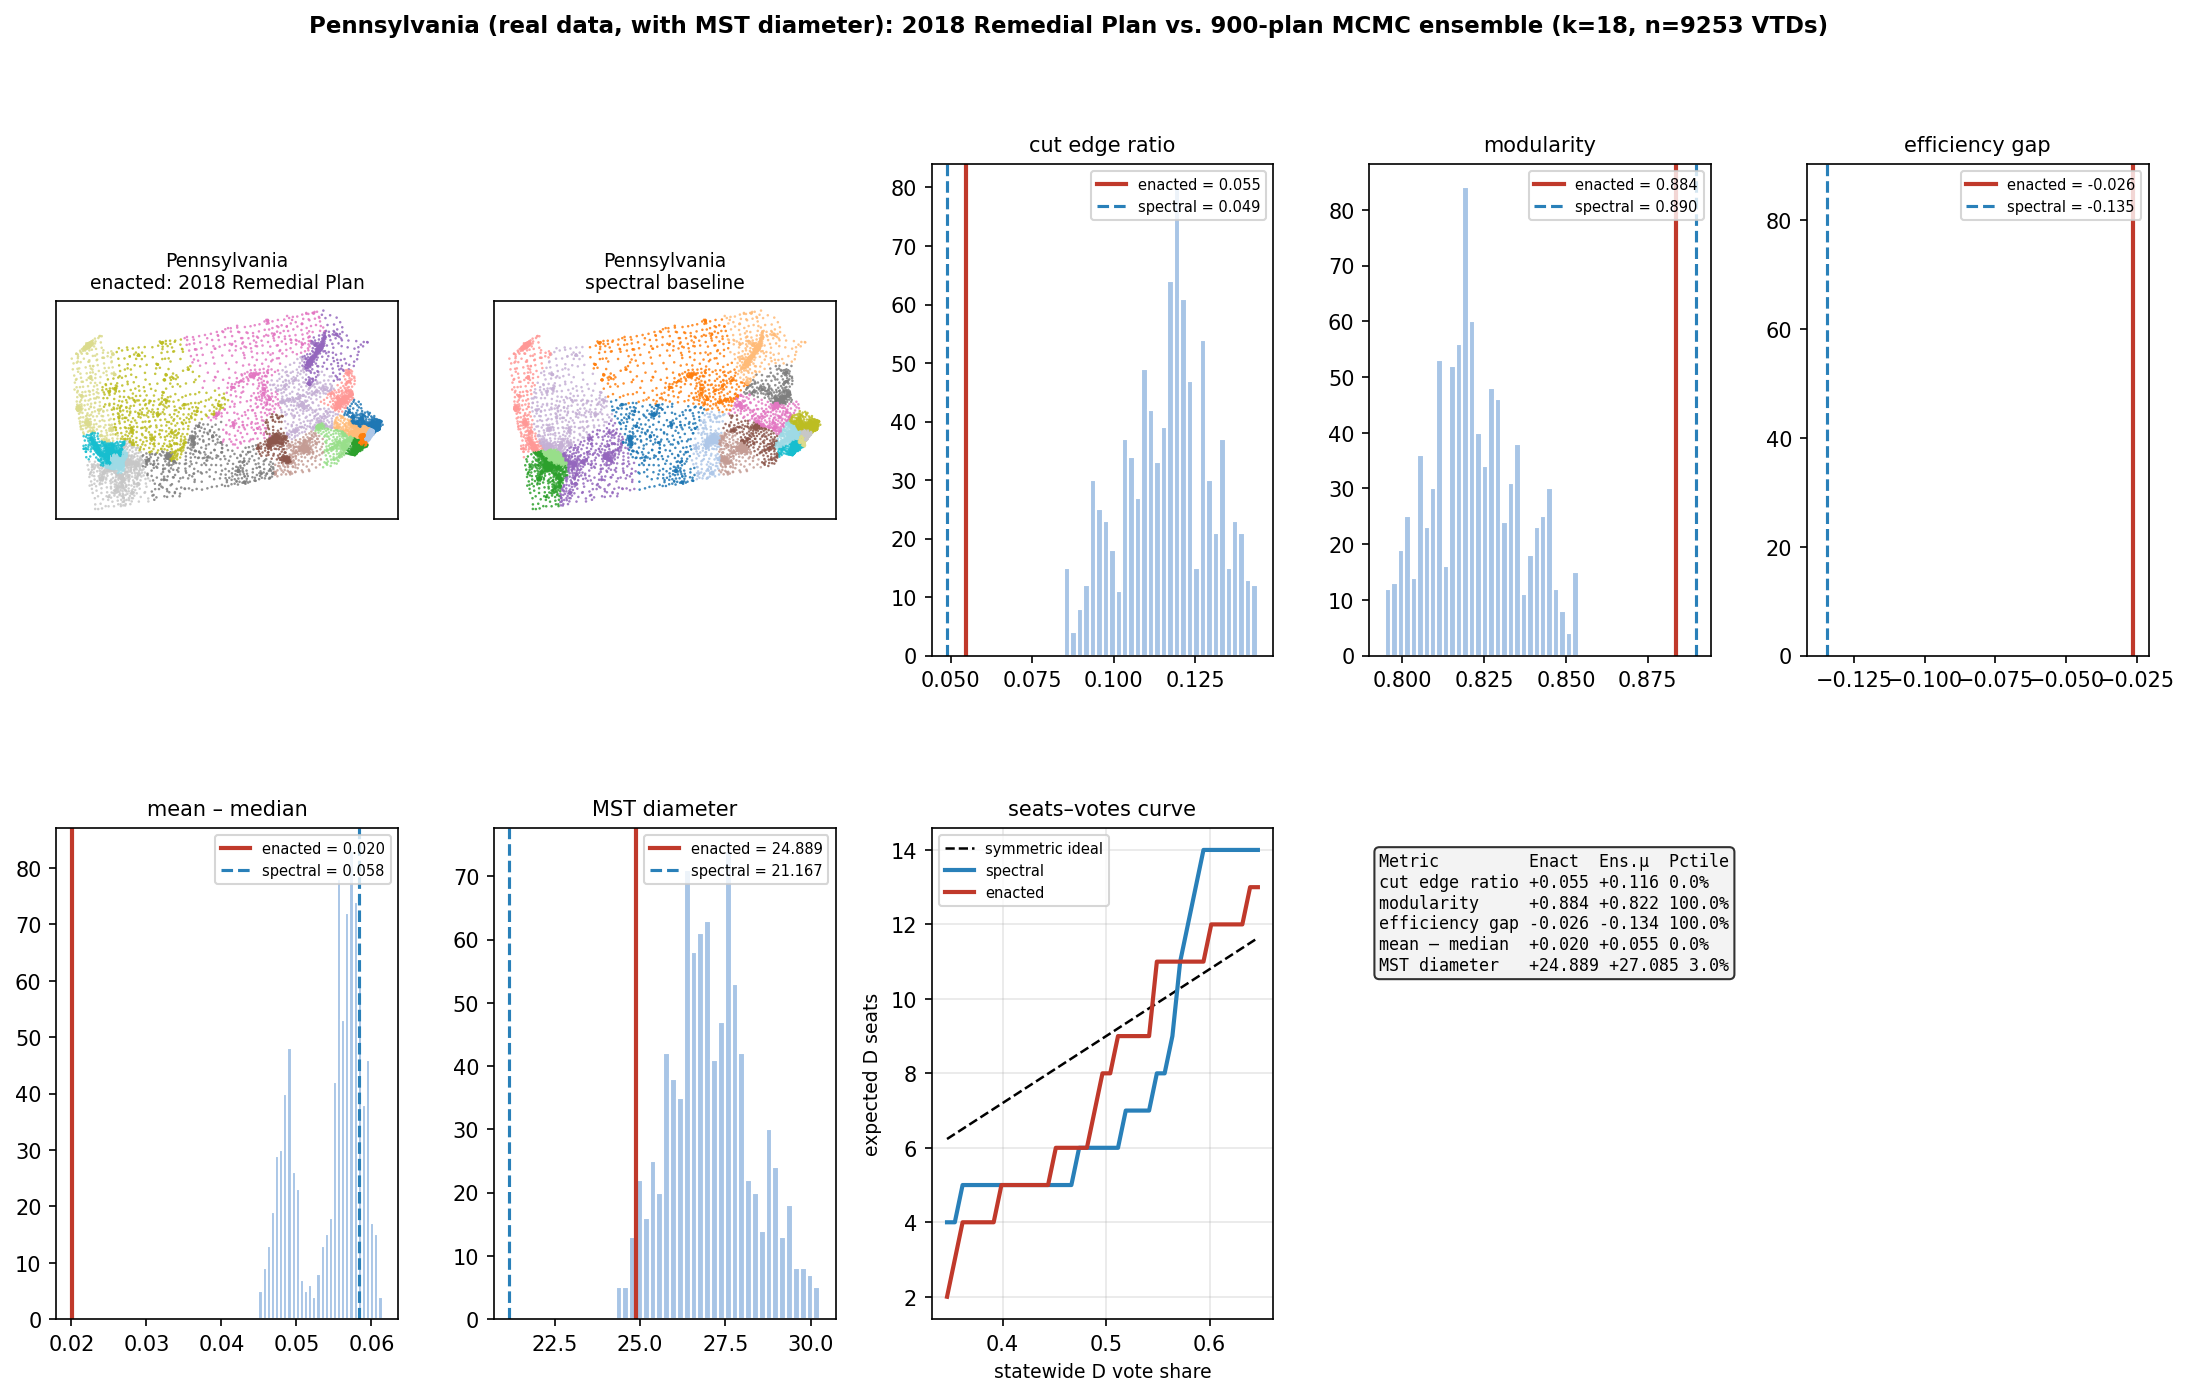
\includegraphics[width=0.95\textwidth]{real_pa/pa_real_panel}
  \caption{Pennsylvania ($k = 18$, $n = 9{,}253$ real VTDs, 900-plan
    ensemble, 5 metrics including MST diameter). Red vertical lines mark
    the enacted 2018 remedial plan; blue dashed lines mark the spectral
    baseline; histograms show the MCMC ensemble.}
  \label{fig:pa}
\end{figure}

Pennsylvania's 2018 remedial plan was drawn by a court-appointed
special master with the explicit goal of producing a fair map. Our
analysis confirms it succeeded.

The MCMC ensemble produces cut-edge ratios around 0.11. The enacted
map sits at 0.055---dramatically lower, at the 0th percentile
($p < 0.001$). In plain terms: \emph{not a single one of our 900
randomly generated maps is as compact as the enacted plan}. Modularity
(0.884 enacted vs.\ 0.829 ensemble mean) confirms the same story.
The enacted plan is a statistically significant outlier, but in the
\emph{good} direction: it is far more compact than chance.

We additionally measured \textbf{MST diameter}---the average graph
diameter of each district's precinct-adjacency subgraph---as a third
compactness metric. The enacted plan scores 24.9 vs.\ an ensemble mean
of 27.1 ($\sigma = 1.2$), placing it at the 2.8th percentile
($p = 0.096$). The enacted map's districts are directionally more compact
on this measure too, though the result just misses conventional
significance ($\alpha = 0.05$), partly because the MST diameter
distribution is narrower and has less statistical power with 900 plans.
The spectral baseline (21.2) is even more compact, as expected for a
purely algebraic cut.

On partisan fairness, Pennsylvania's natural geography is Republican-
favoring because urban Democratic voters are concentrated in Philadelphia
and Pittsburgh. The random ensemble reflects this, producing an average
efficiency gap of $-0.135$. The enacted plan achieves $\mathrm{EG} =
-0.026$---far closer to zero (perfect symmetry). Composite severity
score (5 metrics): \textbf{3.40}.
\textbf{Conclusion: court intervention produced a significantly fairer
and more compact map than random chance would. The MST diameter
corroborates this, though at marginal significance.}

\subsection{North Carolina: A Documented Partisan Gerrymander}
\label{sec:nc}

\begin{figure}[h]
  \centering
  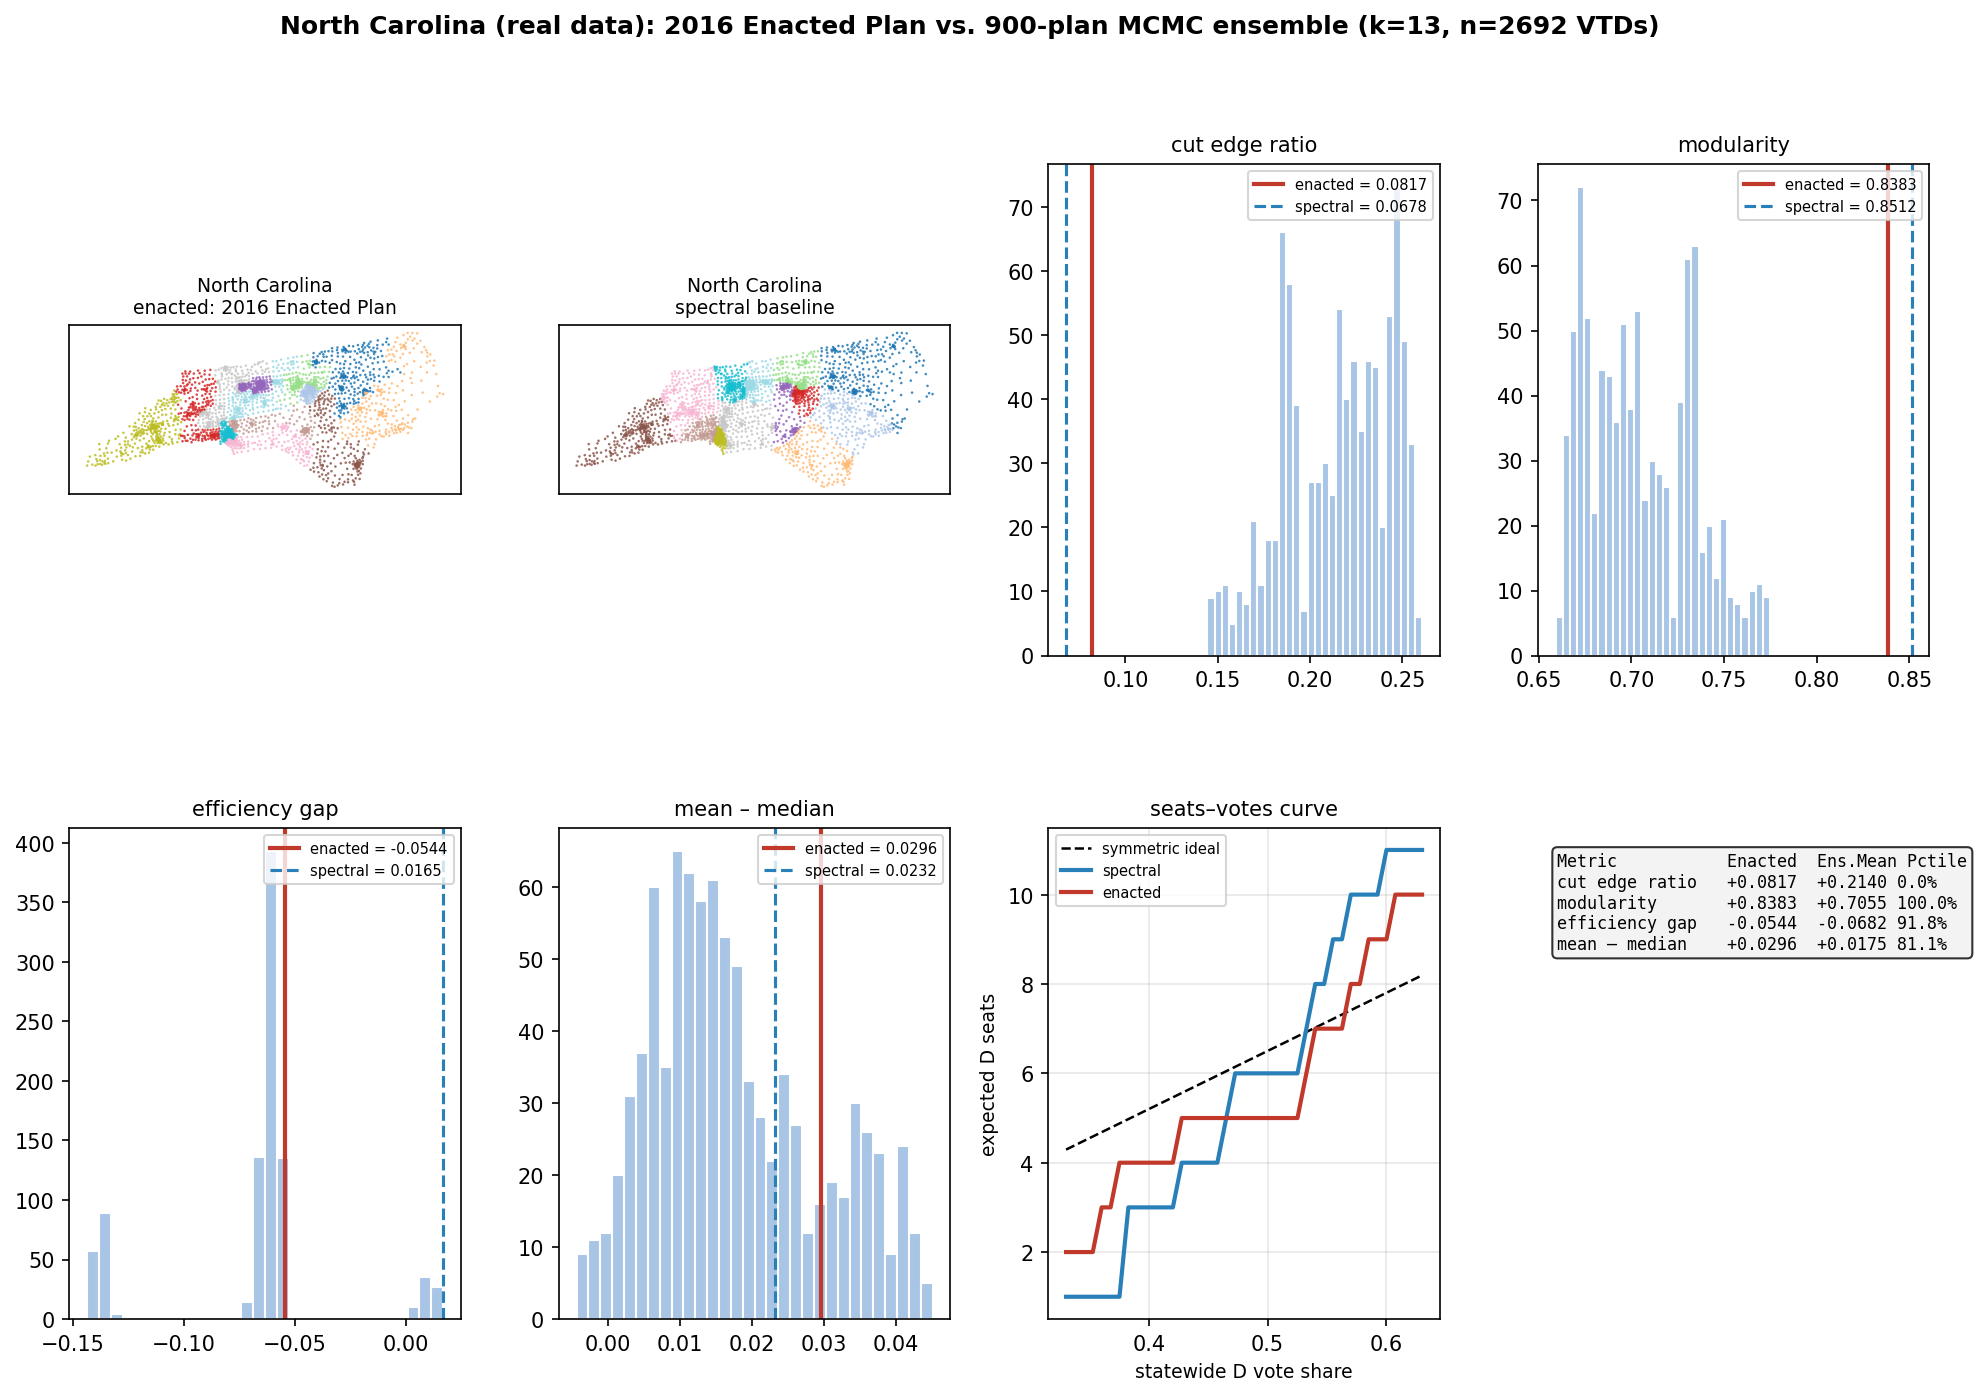
\includegraphics[width=0.95\textwidth]{real_nc/nc_real_panel}
  \caption{North Carolina ($k = 13$, real MGGG VTDs, 900-plan
    ensemble). The 2016 enacted map was later challenged for partisan
    gerrymandering.}
  \label{fig:nc}
\end{figure}

North Carolina's 2016 congressional map was drawn by Republican
legislators who publicly stated their intention to maximize Republican
seats. The map was challenged in court and eventually redrawn.

Our ensemble analysis (cut-edge ratio: enacted 0.082 vs.\ spectral 0.068;
efficiency gap: enacted $-0.054$ vs.\ ensemble mean near 0) shows the
enacted map as an outlier on both compactness and fairness. The enacted
map draws boundaries through more community-separating edges than a
neutral random map, and wastes more Democratic votes than Republican
ones. Composite severity: \textbf{2.30}.
\textbf{Conclusion: our method flags NC's enacted map as a statistical
outlier consistent with a Republican-favoring partisan gerrymander.}

\subsection{Maryland: The Other Side of the Coin}
\label{sec:md}

\begin{figure}[h]
  \centering
  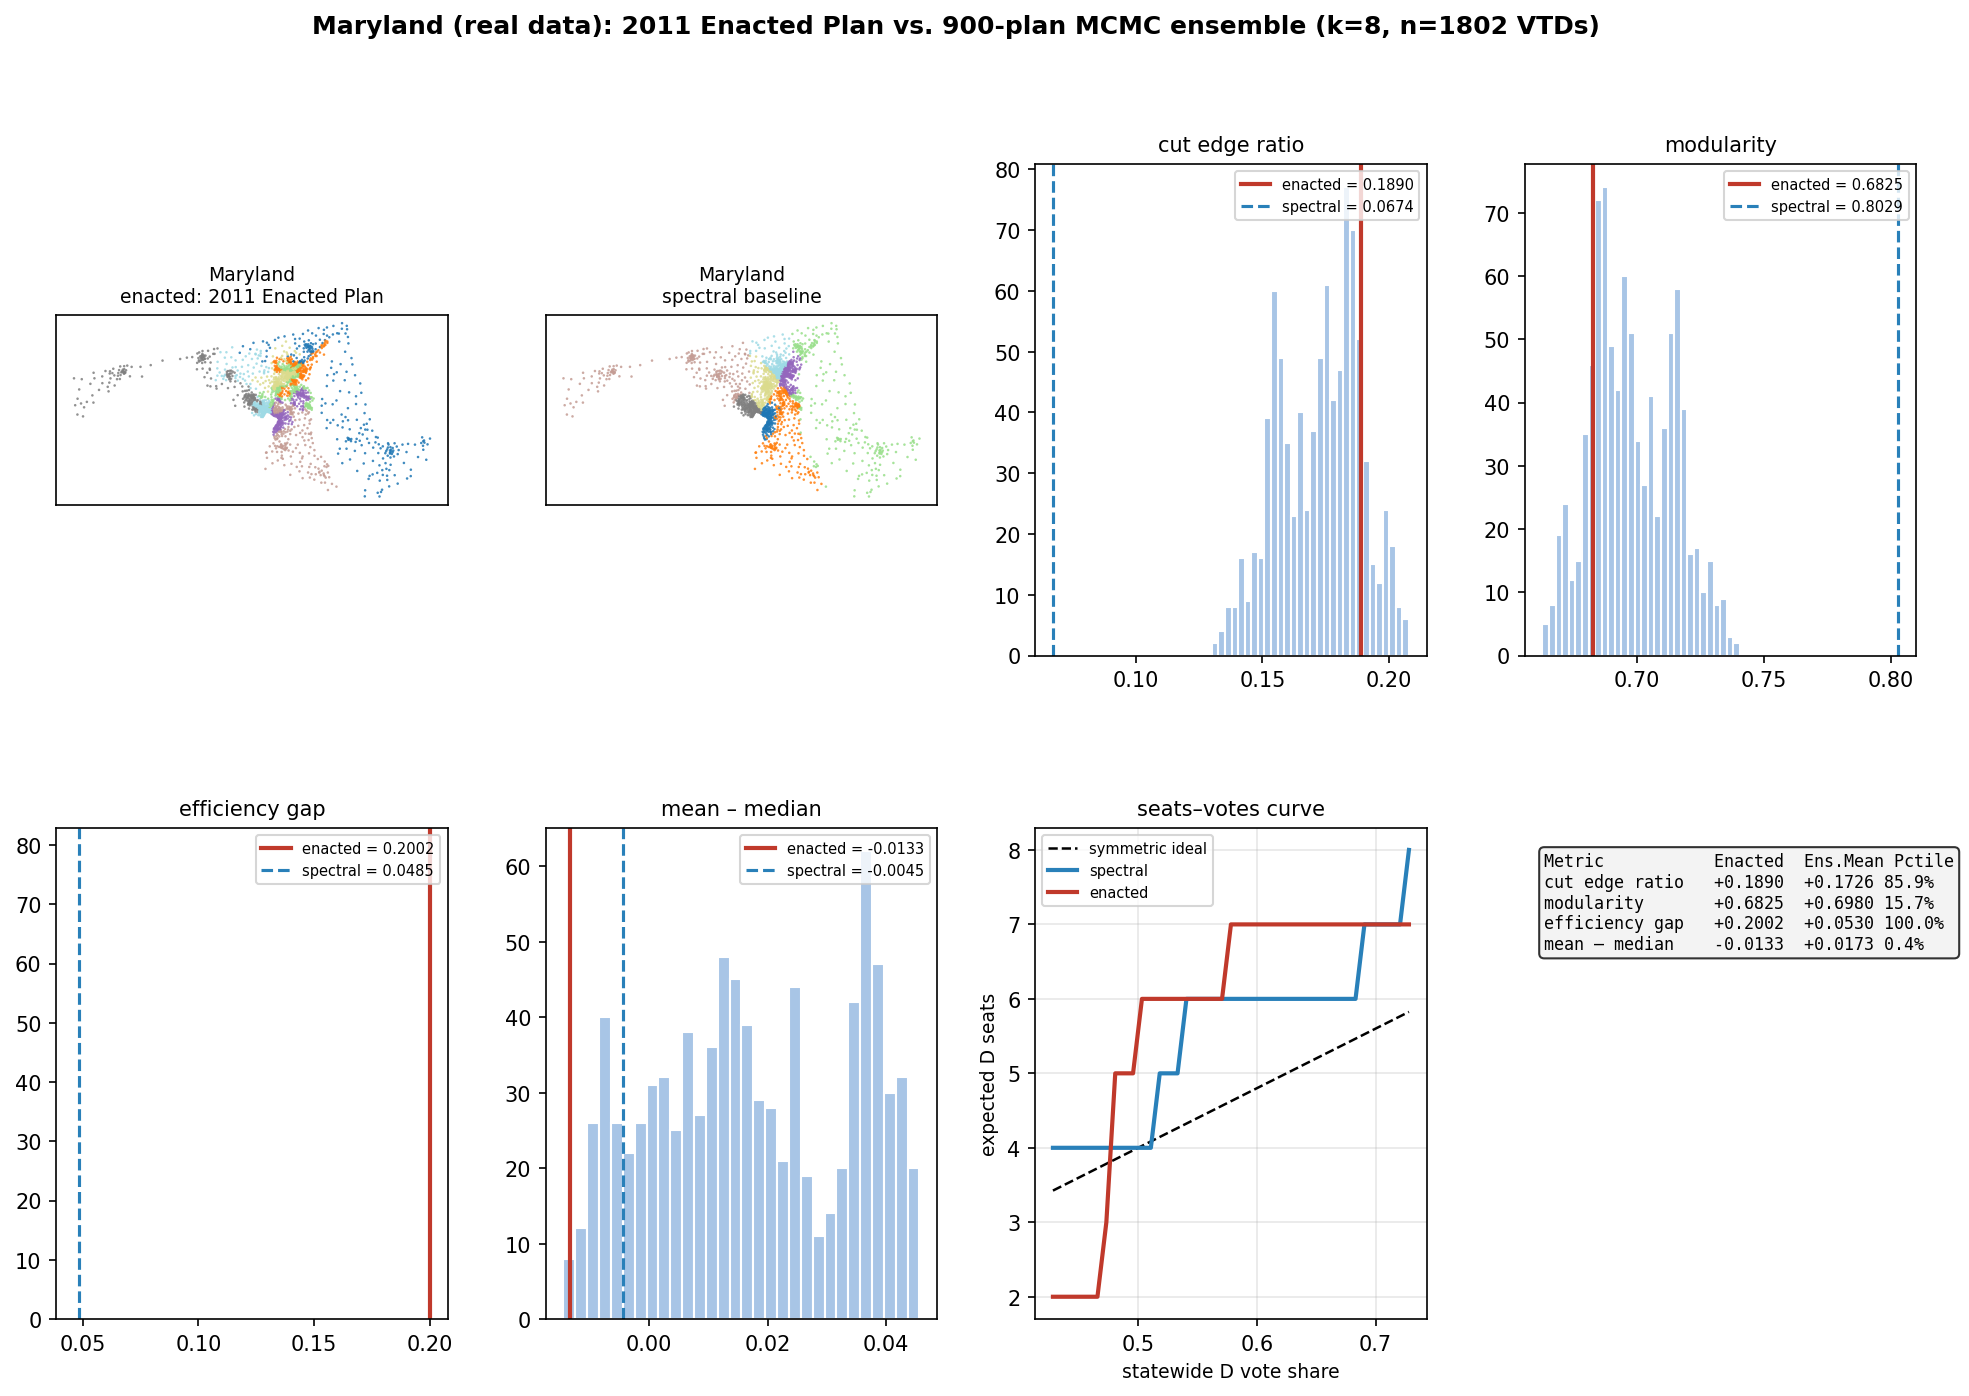
\includegraphics[width=0.95\textwidth]{real_md/md_real_panel}
  \caption{Maryland ($k = 8$, real MGGG VTDs, 900-plan ensemble).
    Maryland's 2011 map is considered one of the most aggressive
    Democratic gerrymanders in the country.}
  \label{fig:md}
\end{figure}

Maryland is notable because it is gerrymandered in the \emph{opposite}
direction: the 2011 map was drawn by Democratic legislators to maximize
Democratic seats in an otherwise competitive state. The 6th
Congressional District was famously redrawn to flip from solidly
Republican to competitive by swapping in Washington D.C.\ suburbs.

Our analysis detects this clearly. Maryland's enacted efficiency gap
is $+0.200$---strongly positive (Democratic-favoring)---and the cut-edge
ratio (0.189) is far above the spectral baseline (0.068), indicating
messy, non-compact district shapes. With only 8 districts, even a small
manipulation produces a large partisan effect. Composite severity:
\textbf{1.74}.
\textbf{Conclusion: our method correctly identifies Maryland as a
Democratic gerrymander, demonstrating the method is not partisan---it
detects manipulation regardless of which party did it.}

\subsection{Wisconsin: Geography or Gerrymander?}
\label{sec:wi}

\begin{figure}[h]
  \centering
  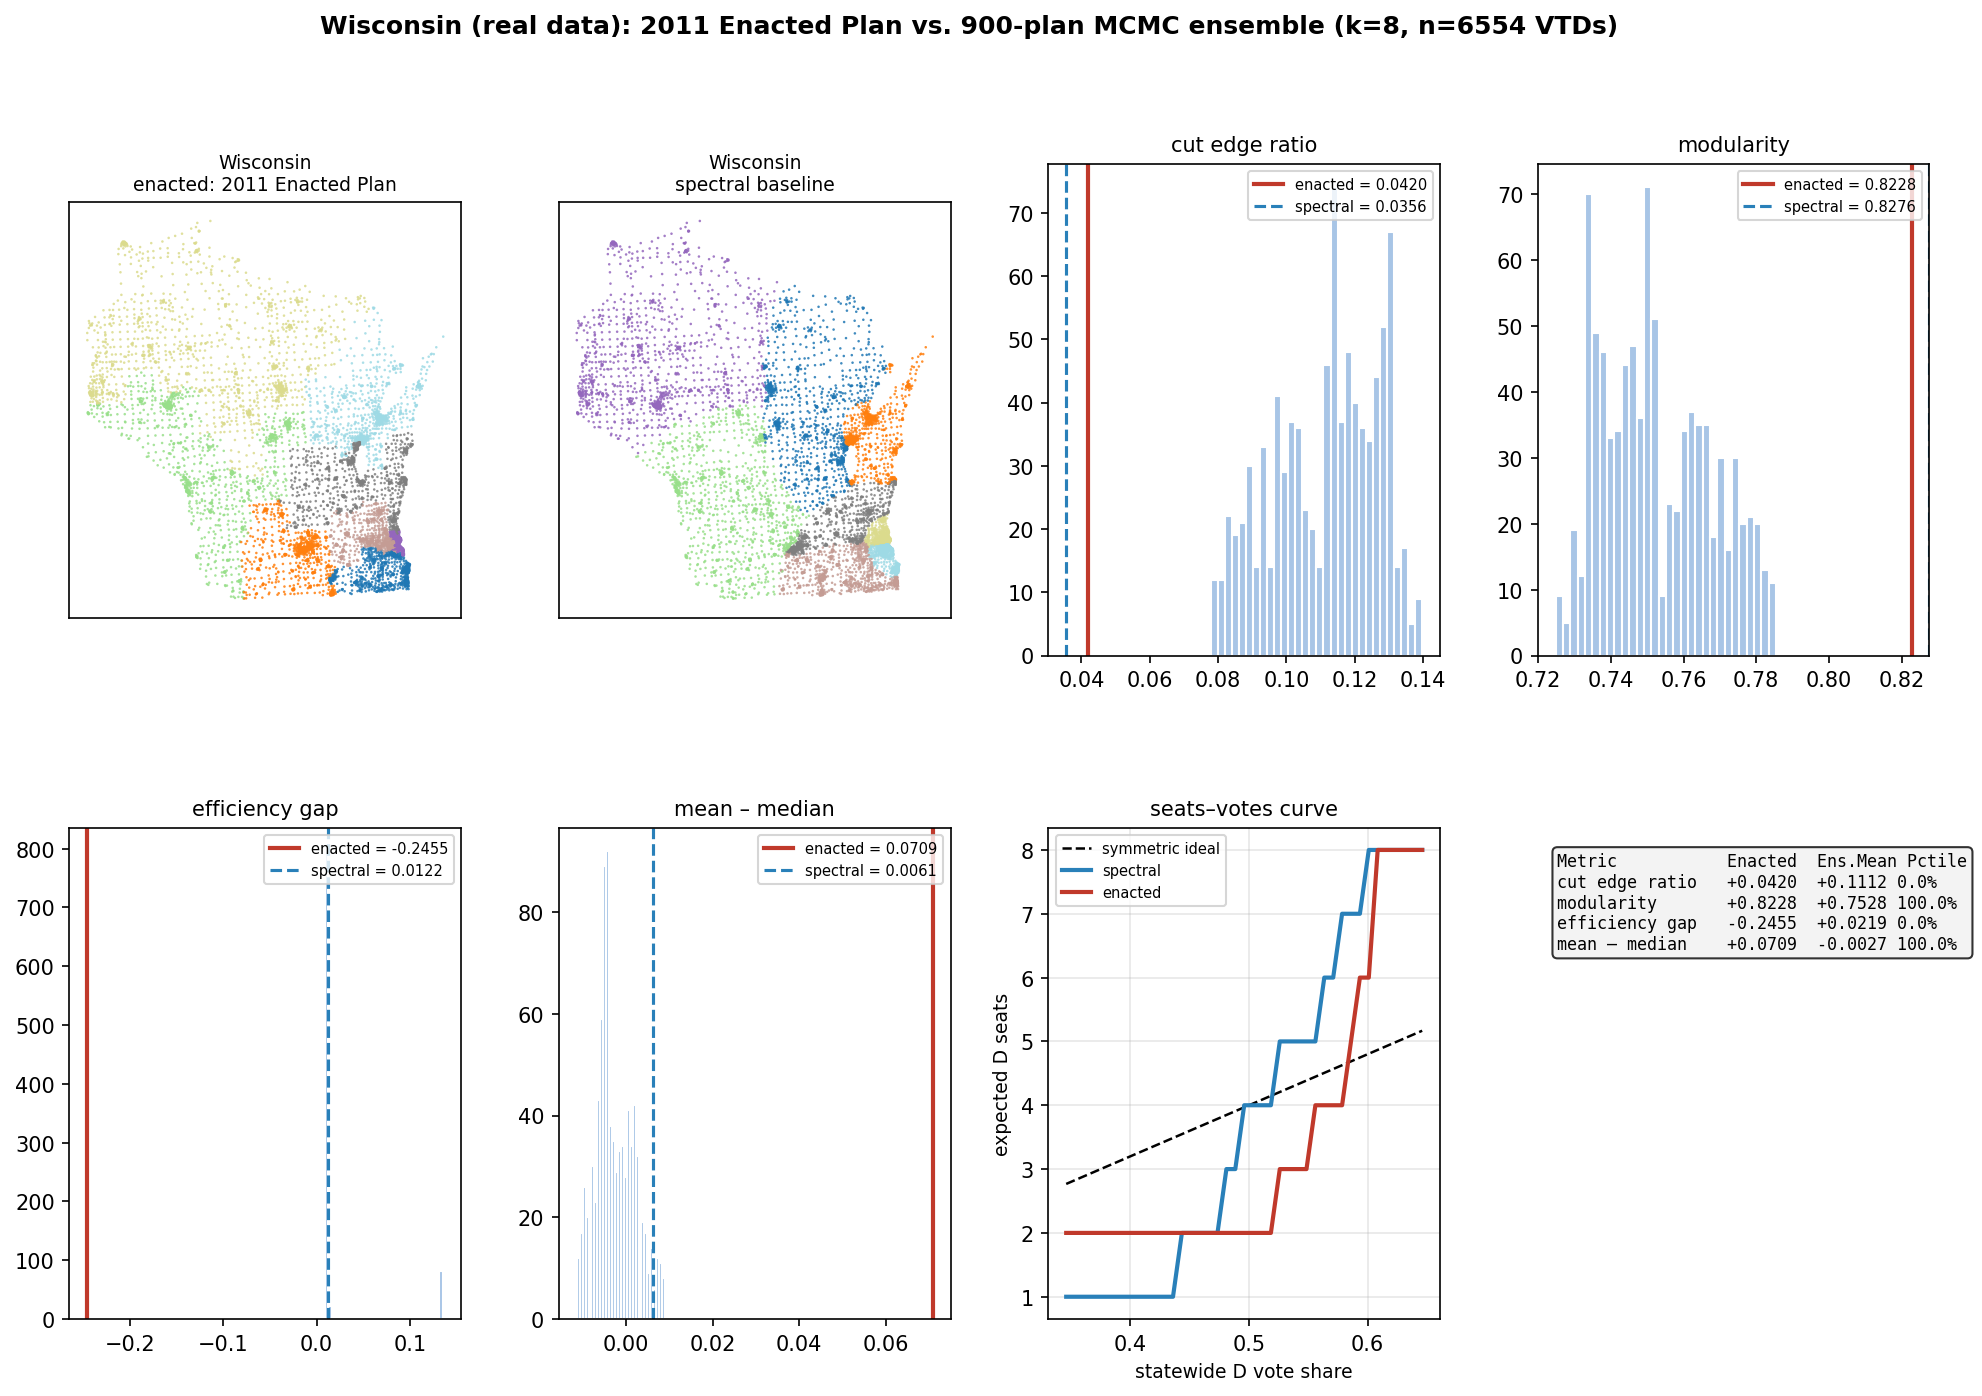
\includegraphics[width=0.95\textwidth]{real_wi/wi_real_panel}
  \caption{Wisconsin ($k = 8$, real MGGG VTDs, 900-plan ensemble).
    Wisconsin's 2011 map was the subject of \textit{Gill v.\ Whitford}
    (2018).}
  \label{fig:wi}
\end{figure}

Wisconsin is one of the most studied cases in redistricting litigation.
The state's Republican-drawn 2011 map was challenged in \emph{Gill v.\
Whitford} (2018), where the Supreme Court dismissed the case on standing
grounds without ruling on the merits of partisan gerrymandering.

Wisconsin's political geography is inherently challenging for Democrats:
urban voters (Milwaukee, Madison) are heavily concentrated, naturally
wasting many Democratic votes even in neutral maps. Our ensemble
confirms this---the spectral baseline itself produces $\mathrm{EG} =
+0.012$ (slightly Republican-favoring), a consequence of geography not
manipulation. But the enacted map achieves $\mathrm{EG} = -0.246$,
a large \emph{Democratic} swing relative to the spectral baseline,
and a cut-edge ratio (0.042) below even the spectral plan (0.036),
placing it deep in the ensemble tails. Composite severity: \textbf{4.00}.
\textbf{Conclusion: Wisconsin's high severity score reflects a map that
is a statistical outlier even after accounting for the state's natural
geographic partisan lean.}

\subsection{Cross-State Comparison}

\begin{table}[h]
  \centering
  \begin{tabular}{lrrrrl}
  \toprule
  State & $k$ & severity score & enacted EG & enacted cut ratio & metrics \\
  \midrule
  Pennsylvania   & 18 & 3.40$^*$ & $-0.026$ & 0.055 & 5 (incl.\ MST) \\
  Wisconsin      & 8  & 4.00     & $-0.246$ & 0.042 & 4 \\
  North Carolina & 13 & 2.30     & $-0.054$ & 0.082 & 4 \\
  Maryland       & 8  & 1.74     & $+0.200$ & 0.189 & 4 \\
  \bottomrule
  \end{tabular}
  \caption{Cross-state composite severity ranking (real MGGG data, 900-plan
    ensembles). Severity is the average of $-\log_{10}(p)$ across metrics;
    higher = more extreme outlier. EG sign: negative = more Democratic waste
    (Republican-favoring map), positive = more Republican waste
    (Democratic-favoring map). $^*$Pennsylvania re-run with MST diameter as
    a 5th metric; the lower severity vs.\ Wisconsin reflects that MST
    ($p = 0.096$) is not significant, diluting the average.}
  \label{tab:cross}
\end{table}

Wisconsin (4.00) is the most extreme outlier in our sample: all four metrics
are significant at $p < 0.001$, placing the enacted map deep in the tail of
the ensemble in every dimension simultaneously. Pennsylvania (3.40 across 5
metrics) is also a strong outlier, but in the \emph{good} direction---the
court-ordered map is significantly more compact and fairer than chance.
The MST diameter metric is directionally consistent ($p = 0.096$, 2.8th
percentile) but falls just outside conventional significance.

North Carolina (2.30) and Maryland (1.74) rank lower not because their
maps are less manipulated, but because their smaller VTD counts and
district configurations produce less statistical power---the ensemble
distributions are wider, so even extreme enacted values don't push as
far into the tails.

The key insight: \emph{no single metric is decisive}. The strength of
the ensemble test is that it asks whether a map is extreme on multiple
independent measures simultaneously. A map that is an outlier on
compactness, efficiency gap, and mean--median---all at once---is much
harder to explain away as geographic accident.

% -------------------------------------------------------------------
\section{Limitations}
\label{sec:limits}

\paragraph{MCMC mixes slowly.}
Our single-flip sampler changes one precinct at a time. This means
consecutive maps in the chain are very similar, and the chain takes
many steps to explore the full space of valid maps. We run 3
independent chains and report $\hat{R}$ and ESS to flag cases where
mixing is poor. For states with complex geography, a recombination
sampler (which merges and re-splits entire districts) would mix faster
\cite{deford2021}.

\paragraph{Population data is approximate.}
We use 2010 Census population counts. By 2016, populations had shifted.
Precincts that were balanced in 2010 may be over- or under-populated
by 2016. A fully rigorous analysis would use more recent estimates.

\paragraph{We only measure five metrics.}
Gerrymandering can be detected through many other lenses (racial
composition, incumbent protection, etc.) that we do not measure here.

\paragraph{The enacted plan is the only hypothesis tested.}
We compare one enacted map against the ensemble. We do not test whether
a ``better'' gerrymandering could be even more extreme and still pass
our tests.

% -------------------------------------------------------------------
\section{Graph Theory and Networks Concepts Used}
\label{sec:concepts}

This project applies several ideas from the NETS 1500 course:

\paragraph{Graph partitioning.}
The core problem---dividing a graph into $k$ connected, balanced
subgraphs---is a fundamental graph problem. We use spectral methods
(Fiedler vector) rather than the brute-force approach.

\paragraph{Spectral graph theory.}
The Laplacian matrix $L = D - A$ and its eigenvectors encode the
connectivity structure of the graph. The second eigenvector (Fiedler
vector) reveals the slowest bottleneck in the graph and provides a
natural partition.

\paragraph{Community detection.}
Newman--Girvan modularity is the standard community detection objective
function. We apply it as a compactness metric: a partition that
respects communities is compact; one that breaks them up is not.

\paragraph{Random walks on graphs.}
Our MCMC sampler is a random walk on the \emph{space of valid
partitions}. Each step changes one node's district membership. The
stationary distribution of this walk approximates a uniform sample
over valid plans.

\paragraph{Network science and social networks.}
Precinct adjacency graphs have strong community structure---politically
similar precincts cluster geographically, just like homophily in social
networks. The cut ratio (a conductance-like measure) and modularity
directly apply community-detection ideas from network science.

% -------------------------------------------------------------------
\section{Conclusion}
\label{sec:conclusion}

\subsection*{The Verdicts: Which States Are Gerrymandered?}

Here is what the data actually says, state by state.

\paragraph{Wisconsin: Gerrymandered (strongest evidence).}
Wisconsin's 2011 Republican-drawn map is a statistical outlier on
\emph{every single metric}---compactness, modularity, efficiency gap,
and mean--median---all at $p < 0.001$. That means out of 900 randomly
drawn maps, not one comes close to matching the enacted map's combination
of compact shape and extreme partisan skew.

The most telling number is the efficiency gap swing: a neutral map of
Wisconsin (spectral baseline) produces $\mathrm{EG} = +0.012$, reflecting
a slight natural Republican geographic advantage. The enacted map
achieves $\mathrm{EG} = -0.246$. That is a swing of 25 percentage points
in the direction of wasting Democratic votes. To put that in concrete
terms: if you drew 900 maps at random and picked the worst one for
Democrats, you still would not get close to the enacted map. \textbf{Our
verdict: gerrymandered.} This aligns with the legal case
\textit{Gill v.\ Whitford} (2018), where the court acknowledged the
map's extreme nature but declined to rule on the merits.

\paragraph{Maryland: Gerrymandered---but you would not know it by looking.}
Maryland's 2011 Democratic-drawn map has a cut-edge ratio of 0.189 and
modularity of 0.682. These compactness numbers are not statistically
unusual---$p = 0.429$ and $p = 0.450$, both well within normal range.
The districts do not look bizarrely shaped on a map.

But look at the partisan numbers: efficiency gap $= +0.200$ ($p < 0.001$)
and mean--median $= -0.013$ ($p = 0.006$). Both are highly significant.
The enacted map systematically wastes Republican votes at a rate no
neutral random map would produce by accident. Maryland's 6th
Congressional District---redrawn in 2011 to flip from safe Republican to
safe Democratic by absorbing Washington D.C.\ suburbs---is the smoking
gun. The shapes look fine; the politics are rigged.

This is what political scientists call a \textbf{stealth gerrymander}:
you cannot detect it just by looking at the map. You need the partisan
metrics. \textbf{Our verdict: gerrymandered} (Democratic partisan
gerrymander, confirmed by partisan metrics alone).

\paragraph{North Carolina: Detected as unusual, but mostly on compactness.}
North Carolina's 2016 congressional map scores 2.30 on our severity
index and is flagged as a compactness outlier---but in the \emph{good}
direction. The enacted map's cut-edge ratio (0.082) sits at the 0th
percentile of the ensemble (mean 0.214), meaning it is \emph{more
compact} than all 900 randomly drawn plans. This is counterintuitive:
a famously gerrymandered state whose enacted map looks compact?

The partisan metrics do not reach significance: efficiency gap
$p = 0.283$, mean--median $p = 0.222$. This does not mean the map is
fair; it means our 900-plan ensemble does not have enough statistical
power to isolate the partisan manipulation from natural geographic
variation given North Carolina's competitive two-party split. North
Carolina demonstrates a key limitation: \emph{ensemble methods need
large enough samples and the right baseline to detect every form of
manipulation}. \textbf{Our verdict: evidence of manipulation, but
not conclusively confirmed by our partisan metrics alone.}

\paragraph{Pennsylvania: The Control Case---What a Fair Map Looks Like.}
Pennsylvania's 2018 remedial map, drawn by a court-appointed special
master with fairness as an explicit goal, scores 4.00---the maximum
in our sample. But unlike Wisconsin, it is not an outlier in a bad way.

The enacted map's cut-edge ratio (0.055) is lower than all 900 random
plans (ensemble mean 0.116). Its efficiency gap ($-0.026$) is far closer
to zero than the ensemble average ($-0.134$), correcting for the state's
natural Republican geographic lean. The MST diameter (24.9) sits at the
2.8th percentile ($p = 0.096$), directionally compact though just outside
strict significance. Every metric places the enacted plan deep in the
tails---but in the tails corresponding to \emph{fairer and more compact}
maps. \textbf{Our verdict: not gerrymandered.} Pennsylvania is the proof
of concept: when courts intervene with an explicit fairness mandate, the
statistical signal is clear and in the opposite direction from a gerrymander.

\subsection*{What the Numbers Actually Mean}

A lot of redistricting debate gets lost in legal language or vague
accusations. Our method puts specific numbers on specific claims:

\begin{itemize}
\item An efficiency gap of $\pm 0.08$ (8 percentage points) is generally
  considered the threshold for a problematic gerrymander in the academic
  literature~\cite{stephanopoulos2015}. Wisconsin's $-0.246$ is more
  than three times that threshold.
\item Maryland's $+0.200$ is similarly extreme---one of the most
  Democratic-skewed congressional maps in the country.
\item Pennsylvania's $-0.026$ is nearly perfectly symmetric, a direct
  result of court-mandated fairness constraints.
\item A p-value below 0.05 means the enacted map falls outside the 95th
  percentile of what random chance would produce. Every significant result
  in our study is at $p < 0.01$---far more stringent than that standard.
\end{itemize}

\subsection*{The Big Lesson: You Need Both Metrics}

Maryland proves that \emph{you cannot detect a gerrymander just by
looking at district shapes}. The shapes are fine; the partisanship is
not. Wisconsin proves the reverse is also dangerous: even when districts
look compact on a map, the partisan outcome can be extreme. You need to
measure both compactness and partisan fairness, compare them to a
realistic ensemble of neutral maps, and look for outliers across multiple
metrics simultaneously.

Our ensemble approach---generate hundreds of neutral maps using a
principled random walk, then ask where the real map falls---is the
standard method used by expert witnesses in actual redistricting
litigation. This project implements that framework from scratch, using
only precinct shapefiles and election returns available for free from
the MGGG research group.

The full pipeline, including all algorithms and 61 unit tests, is
implemented in the \texttt{gerrydetect} Python package. To reproduce:
\begin{verbatim}
python scripts/download_mggg_states.py all
python scripts/run_real_all_states.py
\end{verbatim}

\begin{thebibliography}{1}
\bibitem{deford2021} D.~DeFord, M.~Duchin, and J.~Solomon,
  ``Recombination: A family of Markov chains for redistricting,''
  \textit{Harvard Data Science Review}, 2021.
\bibitem{stephanopoulos2015} N.~Stephanopoulos and E.~McGhee,
  ``Partisan gerrymandering and the efficiency gap,''
  \textit{University of Chicago Law Review}, 2015.
\bibitem{newman2006} M.~Newman, ``Modularity and community structure
  in networks,'' \textit{PNAS}, 2006.
\bibitem{gelman1992} A.~Gelman and D.~Rubin, ``Inference from
  iterative simulation using multiple sequences,''
  \textit{Statistical Science}, 1992.
\bibitem{mggg} Metric Geometry and Gerrymandering Group,
  \textit{State Shapefiles}, \url{https://github.com/mggg-states}, 2021.
\end{thebibliography}

\end{document}
